% Name: Binary search tree with a search path
% Description: The nodes visited while searching for 6 are highlighted, along with the edges taken.
% Tags: BST, binary search tree, search, data structure

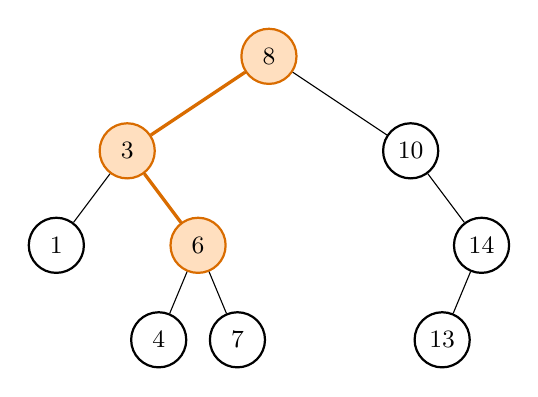
\begin{tikzpicture}[
  level distance=12mm,
  level 1/.style={sibling distance=36mm},
  level 2/.style={sibling distance=18mm},
  level 3/.style={sibling distance=10mm},
  every node/.style={circle, draw, thick, minimum size=7mm, inner sep=0pt, font=\small},
  found/.style={fill=orange!25, draw=orange!85!black},
]
  \node[found] (root) {8}
    child { node[found] (a) {3}
      child { node {1} }
      child { node[found] (b) {6}
        child { node {4} }
        child { node {7} }
      }
    }
    child { node {10}
      child[missing]
      child { node {14}
        child { node {13} }
        child[missing]
      }
    };
  \draw[orange!85!black, very thick] (root) -- (a) -- (b);
\end{tikzpicture}
